\documentclass{standalone}
\usepackage{tikz}
\usetikzlibrary{patterns, positioning}


\begin{document}
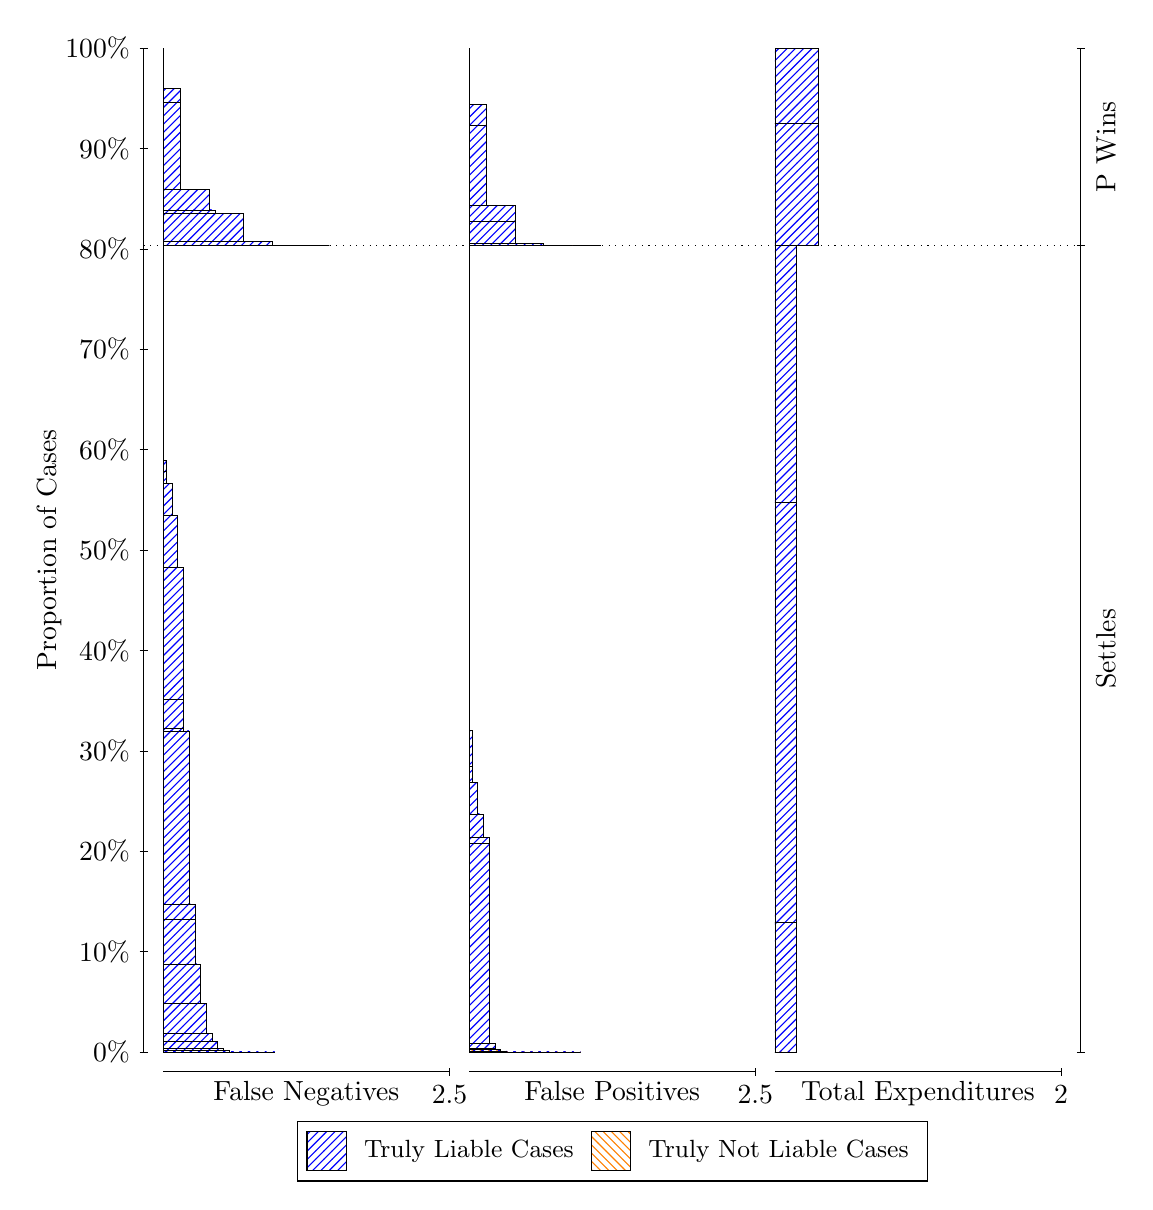
\begin{tikzpicture}
\draw[black, very thin] (1.5,1.75) -- (1.5,14.5);
\node[rotate=90, text=black, anchor=center] at (0.3, 8.125) {Proportion of Cases};
\draw[black, very thin] (1.45,1.75) -- (1.55,1.75);
\node[text=black, anchor=east] at (1.45, 1.75) {0\%};
\draw[black, very thin] (1.45,3.025) -- (1.55,3.025);
\node[text=black, anchor=east] at (1.45, 3.025) {10\%};
\draw[black, very thin] (1.45,4.3) -- (1.55,4.3);
\node[text=black, anchor=east] at (1.45, 4.3) {20\%};
\draw[black, very thin] (1.45,5.575) -- (1.55,5.575);
\node[text=black, anchor=east] at (1.45, 5.575) {30\%};
\draw[black, very thin] (1.45,6.85) -- (1.55,6.85);
\node[text=black, anchor=east] at (1.45, 6.85) {40\%};
\draw[black, very thin] (1.45,8.125) -- (1.55,8.125);
\node[text=black, anchor=east] at (1.45, 8.125) {50\%};
\draw[black, very thin] (1.45,9.4) -- (1.55,9.4);
\node[text=black, anchor=east] at (1.45, 9.4) {60\%};
\draw[black, very thin] (1.45,10.675) -- (1.55,10.675);
\node[text=black, anchor=east] at (1.45, 10.675) {70\%};
\draw[black, very thin] (1.45,11.95) -- (1.55,11.95);
\node[text=black, anchor=east] at (1.45, 11.95) {80\%};
\draw[black, very thin] (1.45,13.225) -- (1.55,13.225);
\node[text=black, anchor=east] at (1.45, 13.225) {90\%};
\draw[black, very thin] (1.45,14.5) -- (1.55,14.5);
\node[text=black, anchor=east] at (1.45, 14.5) {100\%};

\draw[black, very thin] (13.4,1.75) -- (13.4,14.5);
\draw[black, very thin] (13.35,1.75) -- (13.45,1.75);
\node[anchor=west] at (13.35, 1.75) {};
\draw[black, very thin] (13.35,11.989) -- (13.45,11.989);
\node[anchor=west] at (13.35, 11.989) {};
\draw[black, very thin] (13.35,14.5) -- (13.45,14.5);
\node[anchor=west] at (13.35, 14.5) {};

\draw[black, very thin, pattern color=blue, pattern=north east lines] (1.75,1.75) rectangle (3.167,1.75);
\draw[black, very thin, pattern color=blue, pattern=north east lines] (1.75,1.75) rectangle (3.0217,1.75);
\draw[black, very thin, pattern color=blue, pattern=north east lines] (1.75,1.75) rectangle (2.8763,1.75);
\draw[black, very thin, pattern color=blue, pattern=north east lines] (1.75,1.75) rectangle (2.8037,1.75);
\draw[black, very thin, pattern color=blue, pattern=north east lines] (1.75,1.75) rectangle (2.731,1.7502);
\draw[black, very thin, pattern color=blue, pattern=north east lines] (1.75,1.7502) rectangle (2.6583,1.7506);
\draw[black, very thin, pattern color=blue, pattern=north east lines] (1.75,1.7506) rectangle (2.5857,1.7734);
\draw[black, very thin, pattern color=blue, pattern=north east lines] (1.75,1.7734) rectangle (2.513,1.7976);
\draw[black, very thin, pattern color=blue, pattern=north east lines] (1.75,1.7976) rectangle (2.4403,1.8862);
\draw[black, very thin, pattern color=blue, pattern=north east lines] (1.75,1.8862) rectangle (2.3677,1.8874);
\draw[black, very thin, pattern color=blue, pattern=north east lines] (1.75,1.8874) rectangle (2.3677,1.9849);
\draw[black, very thin, pattern color=blue, pattern=north east lines] (1.75,1.9849) rectangle (2.295,2.3677);
\draw[black, very thin, pattern color=blue, pattern=north east lines] (1.75,2.3677) rectangle (2.2223,2.8685);
\draw[black, very thin, pattern color=blue, pattern=north east lines] (1.75,2.8685) rectangle (2.1497,3.4386);
\draw[black, very thin, pattern color=blue, pattern=north east lines] (1.75,3.4386) rectangle (2.1497,3.6321);
\draw[black, very thin, pattern color=blue, pattern=north east lines] (1.75,3.6321) rectangle (2.077,5.827);
\draw[black, very thin, pattern color=blue, pattern=north east lines] (1.75,5.827) rectangle (2.0043,5.8589);
\draw[black, very thin, pattern color=blue, pattern=north east lines] (1.75,5.8589) rectangle (2.0043,6.2263);
\draw[black, very thin, pattern color=blue, pattern=north east lines] (1.75,6.2263) rectangle (2.0043,7.9051);
\draw[black, very thin, pattern color=blue, pattern=north east lines] (1.75,7.9051) rectangle (1.9317,8.5684);
\draw[black, very thin, pattern color=blue, pattern=north east lines] (1.75,8.5684) rectangle (1.859,8.9666);
\draw[black, very thin, pattern color=blue, pattern=north east lines] (1.75,8.9666) rectangle (1.7863,9.1259);
\draw[black, very thin, pattern color=blue, pattern=north east lines] (1.75,9.1259) rectangle (1.7863,9.2632);
\draw[black, very thin, pattern color=orange, pattern=north west lines] (1.75,9.2632) rectangle (1.75,9.2632);
\draw[black, very thin, pattern color=blue, pattern=north east lines] (1.75,9.2632) rectangle (1.75,11.989);
\draw[black, very thin, pattern color=blue, pattern=north east lines] (1.75,11.989) rectangle (3.8573,11.989);
\draw[black, very thin, pattern color=blue, pattern=north east lines] (1.75,11.989) rectangle (3.494,11.99);
\draw[black, very thin, pattern color=blue, pattern=north east lines] (1.75,11.99) rectangle (3.1307,12.041);
\draw[black, very thin, pattern color=blue, pattern=north east lines] (1.75,12.041) rectangle (3.058,12.041);
\draw[black, very thin, pattern color=blue, pattern=north east lines] (1.75,12.041) rectangle (2.7673,12.399);
\draw[black, very thin, pattern color=blue, pattern=north east lines] (1.75,12.399) rectangle (2.6947,12.399);
\draw[black, very thin, pattern color=blue, pattern=north east lines] (1.75,12.399) rectangle (2.404,12.445);
\draw[black, very thin, pattern color=blue, pattern=north east lines] (1.75,12.445) rectangle (2.3313,12.702);
\draw[black, very thin, pattern color=blue, pattern=north east lines] (1.75,12.702) rectangle (2.0407,12.702);
\draw[black, very thin, pattern color=blue, pattern=north east lines] (1.75,12.702) rectangle (1.968,13.811);
\draw[black, very thin, pattern color=blue, pattern=north east lines] (1.75,13.811) rectangle (1.968,13.983);
\draw[black, very thin, pattern color=orange, pattern=north west lines] (1.75,13.983) rectangle (1.75,13.983);
\draw[black, very thin, pattern color=blue, pattern=north east lines] (1.75,13.983) rectangle (1.75,14.5);
\draw[black, very thin, pattern color=orange, pattern=north west lines] (5.6333,1.75) rectangle (7.0503,1.75);
\draw[black, very thin, pattern color=blue, pattern=north east lines] (5.6333,1.75) rectangle (7.0503,1.75);
\draw[black, very thin, pattern color=orange, pattern=north west lines] (5.6333,1.75) rectangle (6.905,1.75);
\draw[black, very thin, pattern color=blue, pattern=north east lines] (5.6333,1.75) rectangle (6.905,1.75);
\draw[black, very thin, pattern color=orange, pattern=north west lines] (5.6333,1.75) rectangle (6.7597,1.75);
\draw[black, very thin, pattern color=blue, pattern=north east lines] (5.6333,1.75) rectangle (6.7597,1.75);
\draw[black, very thin, pattern color=blue, pattern=north east lines] (5.6333,1.75) rectangle (6.687,1.75);
\draw[black, very thin, pattern color=orange, pattern=north west lines] (5.6333,1.75) rectangle (6.6143,1.75);
\draw[black, very thin, pattern color=blue, pattern=north east lines] (5.6333,1.75) rectangle (6.6143,1.75);
\draw[black, very thin, pattern color=blue, pattern=north east lines] (5.6333,1.75) rectangle (6.5417,1.75);
\draw[black, very thin, pattern color=orange, pattern=north west lines] (5.6333,1.75) rectangle (6.469,1.75);
\draw[black, very thin, pattern color=blue, pattern=north east lines] (5.6333,1.75) rectangle (6.469,1.75);
\draw[black, very thin, pattern color=blue, pattern=north east lines] (5.6333,1.75) rectangle (6.3963,1.75);
\draw[black, very thin, pattern color=orange, pattern=north west lines] (5.6333,1.75) rectangle (6.3237,1.75);
\draw[black, very thin, pattern color=blue, pattern=north east lines] (5.6333,1.75) rectangle (6.3237,1.75);
\draw[black, very thin, pattern color=orange, pattern=north west lines] (5.6333,1.75) rectangle (6.3237,1.75);
\draw[black, very thin, pattern color=blue, pattern=north east lines] (5.6333,1.75) rectangle (6.3237,1.75);
\draw[black, very thin, pattern color=blue, pattern=north east lines] (5.6333,1.75) rectangle (6.251,1.7501);
\draw[black, very thin, pattern color=orange, pattern=north west lines] (5.6333,1.7501) rectangle (6.1783,1.7501);
\draw[black, very thin, pattern color=blue, pattern=north east lines] (5.6333,1.7501) rectangle (6.1783,1.752);
\draw[black, very thin, pattern color=blue, pattern=north east lines] (5.6333,1.752) rectangle (6.1057,1.7625);
\draw[black, very thin, pattern color=orange, pattern=north west lines] (5.6333,1.7625) rectangle (6.033,1.7625);
\draw[black, very thin, pattern color=blue, pattern=north east lines] (5.6333,1.7625) rectangle (6.033,1.765);
\draw[black, very thin, pattern color=blue, pattern=north east lines] (5.6333,1.765) rectangle (6.033,1.782);
\draw[black, very thin, pattern color=blue, pattern=north east lines] (5.6333,1.782) rectangle (5.9603,1.7973);
\draw[black, very thin, pattern color=blue, pattern=north east lines] (5.6333,1.7973) rectangle (5.9603,1.862);
\draw[black, very thin, pattern color=orange, pattern=north west lines] (5.6333,1.862) rectangle (5.8877,1.862);
\draw[black, very thin, pattern color=blue, pattern=north east lines] (5.6333,1.862) rectangle (5.8877,4.4039);
\draw[black, very thin, pattern color=blue, pattern=north east lines] (5.6333,4.4039) rectangle (5.8877,4.4758);
\draw[black, very thin, pattern color=blue, pattern=north east lines] (5.6333,4.4758) rectangle (5.815,4.7725);
\draw[black, very thin, pattern color=blue, pattern=north east lines] (5.6333,4.7725) rectangle (5.7423,5.1707);
\draw[black, very thin, pattern color=blue, pattern=north east lines] (5.6333,5.1707) rectangle (5.6697,5.3734);
\draw[black, very thin, pattern color=blue, pattern=north east lines] (5.6333,5.3734) rectangle (5.6697,5.8339);
\draw[black, very thin, pattern color=blue, pattern=north east lines] (5.6333,5.8339) rectangle (5.6333,11.989);
\draw[black, very thin, pattern color=orange, pattern=north west lines] (5.6333,11.989) rectangle (7.3047,11.989);
\draw[black, very thin, pattern color=blue, pattern=north east lines] (5.6333,11.989) rectangle (7.3047,11.989);
\draw[black, very thin, pattern color=orange, pattern=north west lines] (5.6333,11.989) rectangle (6.9413,11.989);
\draw[black, very thin, pattern color=blue, pattern=north east lines] (5.6333,11.989) rectangle (6.9413,11.989);
\draw[black, very thin, pattern color=blue, pattern=north east lines] (5.6333,11.989) rectangle (6.9413,11.989);
\draw[black, very thin, pattern color=orange, pattern=north west lines] (5.6333,11.989) rectangle (6.578,11.989);
\draw[black, very thin, pattern color=blue, pattern=north east lines] (5.6333,11.989) rectangle (6.578,11.997);
\draw[black, very thin, pattern color=blue, pattern=north east lines] (5.6333,11.997) rectangle (6.578,12.017);
\draw[black, very thin, pattern color=orange, pattern=north west lines] (5.6333,12.017) rectangle (6.2147,12.017);
\draw[black, very thin, pattern color=blue, pattern=north east lines] (5.6333,12.017) rectangle (6.2147,12.3);
\draw[black, very thin, pattern color=blue, pattern=north east lines] (5.6333,12.3) rectangle (6.2147,12.506);
\draw[black, very thin, pattern color=orange, pattern=north west lines] (5.6333,12.506) rectangle (6.142,12.506);
\draw[black, very thin, pattern color=blue, pattern=north east lines] (5.6333,12.506) rectangle (6.142,12.506);
\draw[black, very thin, pattern color=blue, pattern=north east lines] (5.6333,12.506) rectangle (5.8513,13.513);
\draw[black, very thin, pattern color=blue, pattern=north east lines] (5.6333,13.513) rectangle (5.8513,13.787);
\draw[black, very thin, pattern color=orange, pattern=north west lines] (5.6333,13.787) rectangle (5.7787,13.787);
\draw[black, very thin, pattern color=blue, pattern=north east lines] (5.6333,13.787) rectangle (5.7787,13.787);
\draw[black, very thin, pattern color=blue, pattern=north east lines] (5.6333,13.787) rectangle (5.7787,13.787);
\draw[black, very thin, pattern color=orange, pattern=north west lines] (5.6333,13.787) rectangle (5.6333,13.787);
\draw[black, very thin, pattern color=blue, pattern=north east lines] (5.6333,13.787) rectangle (5.6333,14.5);
\draw[black, very thin, pattern color=orange, pattern=north west lines] (9.5167,1.75) rectangle (9.7892,1.75);
\draw[black, very thin, pattern color=blue, pattern=north east lines] (9.5167,1.75) rectangle (9.7892,3.3915);
\draw[black, very thin, pattern color=orange, pattern=north west lines] (9.5167,3.3915) rectangle (9.7892,3.3915);
\draw[black, very thin, pattern color=blue, pattern=north east lines] (9.5167,3.3915) rectangle (9.7892,8.734);
\draw[black, very thin, pattern color=orange, pattern=north west lines] (9.5167,8.734) rectangle (9.7892,8.734);
\draw[black, very thin, pattern color=blue, pattern=north east lines] (9.5167,8.734) rectangle (9.7892,11.989);
\draw[black, very thin, pattern color=orange, pattern=north west lines] (9.5167,11.989) rectangle (10.062,11.989);
\draw[black, very thin, pattern color=blue, pattern=north east lines] (9.5167,11.989) rectangle (10.062,13.546);
\draw[black, very thin, pattern color=orange, pattern=north west lines] (9.5167,13.546) rectangle (10.062,13.546);
\draw[black, very thin, pattern color=blue, pattern=north east lines] (9.5167,13.546) rectangle (10.062,14.5);
\draw[black, dotted] (1.5,11.989) -- (13.4,11.989);
\draw[black, very thin] (1.75,1.5) -- (5.3833,1.5);
\node[text=black, anchor=north] at (3.5667, 1.5) {False Negatives};
\draw[black, very thin] (5.3833,1.45) -- (5.3833,1.55);
\node[text=black, anchor=north] at (5.3833, 1.45) {2.5};

\draw[black, very thin] (5.6333,1.5) -- (9.2667,1.5);
\node[text=black, anchor=north] at (7.45, 1.5) {False Positives};
\draw[black, very thin] (9.2667,1.45) -- (9.2667,1.55);
\node[text=black, anchor=north] at (9.2667, 1.45) {2.5};

\draw[black, very thin] (9.5167,1.5) -- (13.15,1.5);
\node[text=black, anchor=north] at (11.333, 1.5) {Total Expenditures};
\draw[black, very thin] (13.15,1.45) -- (13.15,1.55);
\node[text=black, anchor=north] at (13.15, 1.45) {2};

\node[text=black, centered, rotate=90] at (13.72, 6.8695) {Settles};
\node[text=black, centered, rotate=90] at (13.72, 13.245) {P Wins};

\draw (7.449999999999999,1.5) node[draw=none] (baseCoordinate) {};
\begin{scope}[align=center]
        \matrix[scale=0.5, draw=black, below=0.5cm of baseCoordinate, nodes={draw}, column sep=0.1cm]{
            \node[rectangle, draw, minimum width=0.5cm, minimum height=0.5cm, pattern color=blue, pattern=north east lines] {}; &
            \node[draw=none, font=\small, text=black] (B) {Truly Liable Cases}; &
            \node[rectangle, draw, minimum width=0.5cm, minimum height=0.5cm, pattern color=orange, pattern=north west lines] {}; &
            \node[draw=none, font=\small, text=black] (B) {Truly Not Liable Cases}; \\
            };
\end{scope}

\end{tikzpicture}
\end{document}